\documentclass[a4paper]{article}
\usepackage{ makeidx,amsmath, amsthm,amssymb,fancyvrb, multicol}
\usepackage{ graphicx}

\usepackage[top=1.5 cm, bottom=2cm, left=1.5cm, right=1.5 cm]{geometry}
\begin{document}
\begin{center}
\vspace{3cm}
{\bf{\huge Chord book }}\\
\vspace{2cm}
{\bf by Michele Esposito} \\
\vspace{2cm}
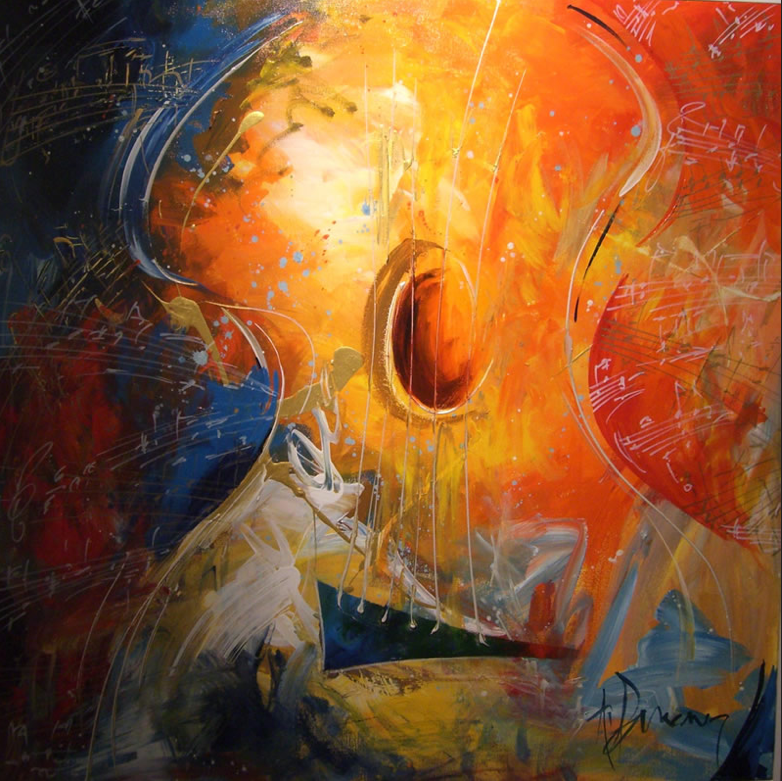
\includegraphics[scale=.6]{guitar2.png}\\
\vspace{1cm}
\emph{A(nother) collection of all the songs I love to play}
\end{center}
\newpage
\tableofcontents
\newpage
\section{Buena Vista Social Club} % (fold)
\label{sec:Buena Vista Social Club}
\subsection{Quizas, Quizas, Quizas} % (fold)
\label{sub:Quizas, Quizas, Quizas}

\begin{Verbatim}[commandchars=\\\{\}]
(introducción en teclado)
RE,MI,FA,MI,FA,RE, SOL, FA,MI,RE,MI,DO,
RE,DO,SI,LA,SOL,LA,SI,DO,RE,
RE,MI,FA,MI,FA,RE, SOL, FA,MI,RE,MI,DO,
RE,DO,SI,LA,SOL,LA

                   Em          Am              Em
Siempre que te pregunto que ¿Cuándo? ¿Cómo? y ¿Dónde?
     Am            Em       F#7     B7      E7
Tu siempre me respondes:  Quizás, quizás, quizás
                 Em    Am         Em     Am
Y así pasan los días y yo desesperando y tú,
        Em        F#7      B7     E7
tú contestando:  Quizás, quizás, quizás.
           B7                        E
Estás perdiendo el tiempo pensando, pensando
                     B7                   E
Por lo que tu más quieras hasta cuando, hasta cuando
                Em     Am         Em     Am
Y así pasan los días y yo desesperando y tú,
         Em        F#7      B7     E7
tú contestando:  Quizás, quizás, quizás.

solo teclado (introducción)

                   Em          Am              Em
Siempre que te pregunto que ¿Cuándo? ¿Cómo? y ¿Dónde?
     Am            Em       F#7     B7      E7
Tu siempre me respondes:  Quizás, quizás, quizás
                 Em    Am         Em     Am
Y así pasan los días y yo desesperando y tú,
         Em        F#7      B7     E7
tú contestando:  Quizás, quizás, quizás.
           B7                        E
Estás perdiendo el tiempo pensando, pensando
                    B7                   E
Por lo que tu más quieras hasta cuando, hasta cuando
                Em     Am        Em       Am
Y así pasan los días y yo desesperando y tú,
          Em        F#7      B7     E7
tú contestando:  Quizás, quizás, quizás.
  F#7      B7     E7
Quizás, quizás, quizás. [bis..(3)]
\end{Verbatim}
\newpage
% subsection Quizas, Quizas, Quizas (end)
% section Buena Vista Social Club (end)
\section{Calle 13} % (fold)
\label{sec:Calle 13}
\subsection{Muerte en Hawaii} % (fold)
\label{sub:Muerte en Hawaii}

\begin{Verbatim}[commandchars=\\\{\}]

Intro: Eb

Eb
Yo he peliao con cocodrilos
                          Bb
Me he balanceado sobre un hilo cargando más de 500 kilos
Cm 
Le he dao la vuelta al mundo en menos de un segundo
Ab                         Bb
He cruzao 100 laberintos y nunca me confundo
Eb
Respiro dentro y fuera del agua como las focas
G7
Soy a prueba de fuego, agarro balas con la boca
Cm
Mi creatividad vuela como los aviones
Ab                             Bb
Puedo construir un cerebro sin leer las instrucciones


Ab                         Bb
Hablo todos los idiomas de todos los abecedarios
Cm
Tengo más vocabulario que cualquier diccionario
Ab                     Bb
Tengo vista de águila, olfato de perro
Cm
Puedo caminar descalzo sobre clavos de hierro
Ab
Soy inmune a la muerte
Cm
No necesito bendiciones porque siempre tengo buena suerte
Ab
Ven conmigo a dar un paseo por el parque
             G7
Porque tengo más cuentos que contarte que García Marqués


Eb
Por ti, todo lo que hago lo hago por ti
                                  Cm
Es que tú me sacas lo mejor de mí

Soy todo lo que soy
          Ab               Bb
Porque tú eres todo lo que quiero (x2)


Eb
Puedo brincar la cuerda con solo una pierna
    Bb
Veo buen la oscuridad sin usar una linterna
Cm
Cocino lo que quieras, yo soy todo un chef
      Ab          Bb
Tengo sexo 24 - 7 todo el mes
Eb
Puedo soplar las nubes grises pa que tengas un buen día
G7
También se como comunicarme por telepatía
Cm
Por ti, cruzo las fronteras sin visa
Ab                            Bb
Y le saco una buena sonrisa a la Mona Lisa


Ab                       Bb
Por ti, respiro antes de morirme
Cm
Por ti voy a la Iglesia y escucho toda la misa sin dormirme
Ab                  Bb
Sigo siendo el Rey, aunque no tenga reino
Cm
Mi sudor huele a perfume y nunca me despeino
Ab                        Bb
Se pelear todas las artes marciales
Cm
También se como comunicarme con los animales
Ab
Mientras más pasa el tiempo me veo más joven
                  G7
Y esta canción la compuse sin escuchar como Beethoven

Eb
Por ti, todo lo que hago lo hago por ti
                                  Cm
Es que tú me sacas lo mejor de mí

Soy todo lo que soy
          Ab               Bb
Porque tú eres todo lo que quiero (x2)
\end{Verbatim}
\newpage
% subsection Muerte en Hawaii (end)
\subsection{La Vuelta al Mundo} % (fold)
\label{sub:La Vuelta al Mu}

\begin{Verbatim}[commandchars=\\\{\}]
Bb
No me regalen mas libros
A7
Por que no los leo 
Dm
Lo que he aprendido es por que lo veo 
         Bb                  A7
Mientras mas pasan los anos me contradigo cuando pienso 
Dm                     G
El tiempo no me mueve yo me muevo con el tiempo 

Soy las ganas de vivir 
las ganas de cruzar 
las ganas de conocer lo que hay despues del mar 
yo espero que mi boca nunca se calle 
tambien espero que las turbinas de este avion nunca me fallen 
no tengo todo calculado ni mi vida resuelta 
solo tengo una sonrisa y espero una de vuelta
yo confio en el destino y en la marejada 
yo no creo en la iglesia pero creo en tu mirada 
tu eres el sol en mi cara cuando me levanta 
yo soy la vida que ya tengo tu eres la vida que me falta 
asi que agarra tu maleta el bulto los motetes 
el equipaje tu valija la mochila con todos tus juguetes y 

B....                   A7....            Dm....
dame la mano y vamos a darle la vuelta al mundo darle la vuelta al mundo 
G....
darle al vuelta al mundo 
B....                   A7....            Dm....
dame la mano y vamos a darle la vuelta al mundo darle la vuelta al mundo 
G....
darle al vuelta al mundo 

la renta el sueldo el trabajo en la oficina 
lo cambie por las estrellas y por huertos de harina 
me escape de la rutina para pilotear mi viaje 
por que el cubo en el que vivia se convirtio en paisaje 
yo era un objeto esperando a ser ceniza 
un dia decidi hacerle caso a la brisa 
a irme resbalando detras de tu camisa 
no me convencio nadie me convencio tu sonrisa 
y me fui tras de ti persiguiendo mi instinto 
si quieres cambio verdadero pues camina distinto 
voy a escaparme hasta la constelacion mas cercana la suerte es mi oxigeno tus ojos son mi ventana 
quiero correr por 7 lagos en un mismo dia 
sentir encima de mis muslos el clima de tus nalgas frias 
llegar al tope de la sierra abrazarme con las nubes 
sumergirme bajo el agua y ver como las burbujas suben y

dame la mano y vamos a darle la vuelta al mundo darle la vuelta al mundo darle al vuelta al mundo 
dame la mano y vamos a darle la vuelta al mundo darle la vuelta al mundo darle al vuelta al mundo
\end{Verbatim}
\newpage
% subsection La Vuelta al Mu (end)
% section Calle 13 (end)
\section{Renato Carosone} % (fold)
\label{sec:Renato Carosone}
\subsection{Tu Vuo' Fa' L'Americano} % (fold)
\label{sub:}
\begin{Verbatim}[commandchars=\\\{\}]
Lam                         Rem   Mi7           Lam
Puorte 'e cazune cu nu stemma arreto 
 Lam                      Rem  Mi7      Lam         
Na cuppulella cu 'a visiera aizata 
Rem                                             Lam
Passe scampanianno pe' Tuleto,
Si7                                                          Mi7                                          
comm'a nu guappo, pe' te fá guardá! 
                                 Lam
Tu vuo' fá ll'americano,
Siente a me chi t''o ffa fá?
mericano, 'mericano 
Tu vuoi vivere alla moda,
                                          Mi7
po' te siente 'e disturbá 
ma se bevi "Whisky and Soda",
Tu abballe 'o "Rock and Roll",
                                       Lam
tu giochi a "Base Ball "
                           Rem
Ma 'e solde p''e Ccamel,
                       Lam
chi te li dá?
                      Si7
La borsetta di mammá!?
               Mi7
Tu vuó' fá ll'americano,
             Fa7                  Mi7
mericano, mericano,
                                 Lam
            La7       Rem
ma si' nato in Italy!
                                                Lam
Siente a me: Nun ce sta niente 'a fá 
     Fa7     Mi7 Lam
Okay, Napolitan!
               Mi7            Lam
Tu vuó' fá ll'american!
               Mi7            Lam
Tu vuó' fá ll'american!

Comme te pò capí chi te vò' bene,
si tu lle parle miezo americano?
Quanno se fa ll'ammore sott''a luna,
comme te vene 'ncapa 'e dí "I love you"?
Tu vuo' fá ll'americano,
mericano, 'mericano 
ma si' nato in Italy!
Siente a me: Nun ce sta niente 'a fá 
Okay, Napolitan!

Tu vuó' fá ll'american!
Tu vuó' fá ll'american!
Whisky and soda e rock and roll
Whisky and soda e rock and roll
\end{Verbatim}
\newpage
% subsection  (end)
% section Renato Carosone (end)
\section{Eva Cassidy} % (fold)
\label{sec:Eva Cassidy}
\subsection{Somewhere Over The Rainbow} % (fold)
\label{sub:Somewhere Over The Rainbow}
\begin{Verbatim}[commandchars=\\\{\}]
Intro:   C  G Em Am D G

G   G     Bm       Bm
Somewhere over the rainbow
C   Cm     G    G7
    Way up high
C       Cm   G           Em
There's a    land that I heard of
Am        D    G   G
Once in a lullaby


G   G     Bm       Bm
Somewhere over the rainbow
C   Cm        G    G7
    Skies are blue
C   Cm  G               Em      Am
And the dreams that you dare to dream
       D       G    G
Really do come true


G                   G
Some day I'll wish upon a star
    C                 Cm             Em Em  Em
And wake up where the clouds are far behind me
      G                  G
Where troubles melt like lemondrops
 F#7           F#7
Away above the chimney tops
       Bm    Bm     Am   D
That's where you'll find me

G   G     Bm       Bm
Somewhere over the rainbow
C   Cm        G    G7
    Bluebirds fly
C     Cm  G        Em
Birds fly over the rainbow
Am           D         G   G
Why then, oh why can't I?

G                   G
Some day I'll wish upon a star
    C                 Cm             Em Em  Em
And wake up where the clouds are far behind me
      G                  G
Where troubles melt like lemondrops
 F#7           F#7
Away above the chimney tops
       Bm    Bm     Am   D
That's where you'll find me

G   G     Bm       Bm
Somewhere over the rainbow
C   Cm        G    G7
    Bluebirds fly
C     Cm  G        Em
Birds fly over the rainbow
Am           D         G   G
Why then, oh why can't I?

  G             G7
If happy little bluebirds fly
  C
Beyond the rainbow
Am      D        G
Why, oh why can't I?
\end{Verbatim}
% subsection Somewhere Over The Rainbow (end)
\newpage
% section Eva Cassidy (end)
\section{The Cat Empire} % (fold)
\label{sec:The Cat Empire}
\subsection{The Chariot} % (fold)
\label{sub:The Chario}
\begin{Verbatim}[commandchars=\\\{\}]
           Verse 1:
Em                        G
This is a song that came upon me one night 
          Am
When the news it had been telling me 
       C                D
About one more war and one more fight
      Em 
And 'aeh' I sighed but then
     G
I thought about my friends
         Am
Then I wrote this declaration
         C              D
Just in case the world end
 


           Verse 2:
Our guns
Em             G
 We shot them in the things we said
        Am
Ah we didn't need no bullets 
         C            D
Cos we rely on some words instead 
Em
Kill someone in argument
G
Outwit them with our brains 
          Am
And we'd kill ourselves laughing
         C                D
At the funny things we'd say 



           Verse 3:
And bombs 
Em              G
  We had them saved for special times
          Am
When the crew would call a shakedown 
     C            D
We break down a party landmine 
Em
Women that so sexy 
        G
They explode us with their looks 
         Am
Ah we blowing up some speakers 
          C              D        
Jumping round till the ground shook 



           Verse 4:
And missiles
Em                   G
   They were the roadtrips that we launched
       Am
T-t-tripping across this island 
            C              D
Starting missions at the break of dawn
 Em
Yawn and smile say 
        G
What direction shall we take? 
Am
Somewhere where it warm and wet 
C                        D
This be the route we'd always take and 



           Chorus:
Am                      Em
  Our weapons were our instruments 
G           D          C
Made from timber and steel 
              Am
We never yielded to conformity 
      Em
But stood like kings 
        G
In a chariot that's riding on a 
   D
Record wheel 

            Verse 5:
           Em
And our airforce flying 
            G
When the frisbee in the sky 
         Am
Have a session while we're smoking
             C           D
Now we're feeling extra high 
          Em 
And we'd sneak into a carpark
            G
With the skaties on our back 
            Am
And we're flying down the levels howling 
         C                D
On the attack now on the attack



           Verse 6:
And battles 
Em                   G
  They happened in these dancehalls 
           Am
See we'd rather fight with music
    C               D
Choosing one the rhythm war
Em
Battle at these shakedowns 
         G
And we battle at these gigs 
        Am
We do battle in our bedrooms 
            C                D
Made some sweet love to the beat 



           Bridge:
           Em
Then our allies grew 
     G
Wherever we would roam 
        Am 
See whenever we're together 
        C             D
Any stranger feel at home 
      Em
In a way we are an army 
          G
But this army not destruct 
      Am
No instead we're doing simple things
       C             D
Good loving find it run amuck 



           Verse 7:
Em
This be a declaration 
   G
Written about my friends
        Am
It's engraved into this song 
         C               D
So they know I'm not forgetting them 
      Em
See maybe if the world contained
 G
More people like these 
          Am
Then the news would not be telling me
       C                   D
About all that warfare endlessly and

 Chorus:
\end{Verbatim}
\newpage
% subsection The Chario (end)
\subsection{The Lost Song} % (fold)
\label{sub:The Lost Song}
\begin{Verbatim}[commandchars=\\\{\}]
Dm    Bb    F    Am7
 
the words go a little like this... 
 
VERSE 1: 
    Dm                                        Bb 
Oh, I had nine lives but I lost all of them 
              F 
And I've been searching in the night  
                         Am7 (and so on)...       
And I've been searching in the rain 
I tried to find them, but they disappeared 
They walked away, they dressed in black 
They left my side and all I say is 
That I wasted time when I looked for them 
For now I know that things gone past  
Are never to be found again 
No never, never again 
I had nine lives but lost all of them... 
 
VERSE 2: 
I had a plan but never finished it 
And I've been searching for the thought 
And I've been searching in a haze  
I try all days, to remember it 
But now the blueprint in my mind has gone 
My mind forgot the colour of direction 
And my eyes they see the hands 
That could've built that could've constructed 
The empire in my mind 
The empire I'll never find 
I had a plan but that was where it ended....ended..... 
 
Depending on what version you have, various sections get repeated...
I'm sure you can work it out.
\end{Verbatim}
\newpage
% subsection The Lost Song (end)
\subsection{The Wine Song} % (fold)
\label{sub:The Wine Song}
\begin{Verbatim}[commandchars=\\\{\}]
INTRO
(3/4 time)
| Dm | F+/C# | F | G/B | Bb | 
Dm/A | A7 | Dm |

Dm        F+/C#    F        G/B
Songs and melodies change and change
Bb
And sway
         Dm/A           E7/Ab      A7
But they still stay the same
Dm                F+/C#         G/C       G/B
The songs that we sung when the dark days come
        Bb            Dm/A         A7          Dm
Are the songs that we sung when we chased them away
Dm        F+/C#   F    G/B
If I ever found a pot of gold
        Bb        Dm/A        E7/Ab         A7
I'd buy bottles untold of the nectar of the vines
Dm           F+/C#      F           G/B
I'm going to die with a twinkle in my eye
         Bb              Dm/A          A7            
    Dm
'cause I sung songs spun stories loved laughed and drank wine

Gm       Dm    A7   Dm
Tomorrow is another day
Gm           Dm     A7       Dm
The cats are out to play, to play
     Gm        Dm        A7       Dm
That old rusty spaceship wants to sail
Gm       Dm    A7  Dm
Into the milky way again
     Dm       Abdim   A7     | /A /B 
/C# |
On a river of red red wine

[For this section, its really just the four chords written, but I included the bass 
notes as at the start when it is slow, those are very pronounced. But its just the chords 
with that Jewish Hora feel by alternating between the 5ths]

Dm   Dm/A (repeat)
Run...
(let's have some)
Gm  Gm/D (repeat)
Fun...
(we'll)
Dm   Dm/A (repeat)
Drink...
(a toast to the)
A7   A7/E  (repeat)
Sun...

[Same chords as verse 1]

In summer the bushfires rage and rage
And rage
On such beautiful days
And we fight them with water that runs through the cracks
Water we're desperately trying to save
So I'll just live on wine and water my vines
And sleep on the wind with the fires right behind
And sing on the beaches and dance through the night
Oh we'll cry 'pass the wine, pass the wine, pass the wine'

Gm       Dm    A7   Dm
Tomorrow is another day
Gm           Dm     A7       Dm
The cats are out to play, to play
     Gm        Dm        A7       Dm
That old rusty spaceship wants to sail
Gm       Dm    A7  Dm
Into the milky way again
     Dm       Abdim   A7     | /A /B 
/C# |
On a river of red red wine

[Again, same chords as before]

Run...
(let's have some)
Fun...
(we'll)
Drink...
(a toast to the)
Sun...

[Instrumental solo. This part is the same chords as the "run run run" section. The 
tricky part is the melody line, which I wont include, but if anyone actually wants it just 
contact me]

F         C         A7  Dm
Oh what a beautiful day today!
Gm        F      C    F
Today's a day to celebrate
F         C       A7        Dm
Grab your bucket, grab your spade
Gm            F       C         F
We're heading down to Half Moon Bay
F       C        A7     Dm
I saw a plane go into a cloud
Gm            F         C           F
I'm drunk I'm happy I'm singing and loud
F                  C         A7  Gm   A7  Bb
                            [where the leading melody is C# D E D]
Two o'clock in the arvo, but hey that's allowed...
Gm                F         | C     C/E | F 
          A7 Dm
I'm having a good time and of that I am proud
\end{Verbatim}
\newpage
% subsection The Wine Song (end)
% section The Cat Empire (end)
\section{Dire Straits} % (fold)
\label{sec:Dire Straits}
\subsection{Lions} % (fold)
\label{sub:Lions}
    	  
\begin{Verbatim}[commandchars=\\\{\}]
Intro:  Bm7  D  A  G   Bm7  D  A  G   Bm7  Bm7  Bm7  F# C9 (Stop) 
Bm7     D        A         G9 
Red sun, go down way over dirty town 
Bm7             D             A       E9 
Starlings are sweeping around crazy shoals 
Bm7         D                   A                          G9 
Yes, and a girl is there, high heeling across the square 
Bm7                 D                          A              E9 
The wind it blows around in her hair, and the flags upon the poles 
Em9 
Waiting in the crowd to cross at the light 
                     G     F#m7          Bm7   F#m7   Bm7   F#   C9 
She looks around to find a face she can like. 
Bm7          D           A                        G9 
Church bell, clinging on, trying to get a crowd, Evensong 
Bm7                D        A              E9 
Nobody cares to depend upon, the chime it plays 
Bm7                        D                   A                   G9 
They're all in the station, praying for trains, the congregation's, late again 
Bm7                 D             A                E9 
It's getting darker, all the time, these flagpole days 
Em9 
Drunk old soldier he gives her a fright 
                 G      F#m7   Bm7   F#m7   Bm7   F#   C9 
He's crazy lion howling for a fight. 
Bm7           D               A                    G9 
Strap hanging, gunshot sound, door slamming on the, overground 
Bm7                D              A                 E9 
The starlings are tough, but the lions are made of stone 
Bm7                   D          A                               G9 
Her evening paper is horror torn, but there's hope later for, capricorns 
Bm7                       D           A              E9 
Her lucky stars give her just enough, ... to get her home 
Em9 
Then she's reading about a swing to the right 
                              G     F#m7   Bm7   F#m7   Bm7   F#   C9 
But she's thinking about a stranger in the night 
G                       A    G                        A 
I'm thinking about the lions, I'm thinking about the lions 
G                     A       Bm7   F#m7    Bm7   F#m7    Bm7   F#m7    Bm7 
A   fade out 
What happened to the lions, tonight       (tonight)    (tonight) 
\end{Verbatim}
\newpage
% subsection Lions (end)
\subsection{Wild West End} % (fold)
\label{sub:Wild West E}
\begin{Verbatim}[commandchars=\\\{\}]
D                D            Em               G
 Steppin' out to Angellucci's, for my coffee beans
D                 D      Em           G
 checking out the movies, and the magazines
D             D          Em                         G
 waitress she watches me, crossing from the Barocco bar
D              D     Em       G
 I'm getting a pickup, for my steel guitar
           D           D   Em           G
 I saw you walking out,      Shaftsbury Avenue
D          D                Em      G
 excuse me talking, I wanna   marry you
D        D                        Em                  G
 this is seventh heaven street to me, don't you be so proud
D                    D      Em       G
 You're just another angel,   in the crowd. 

             D              D         Em        G
	And I'm walking in the wild west end
     D              D         Em        G
	Walking in the wild west end
     D                 D         Em        G     D/A G/C /C D/
	Walking with your wild best friend


And my conductress on the number nineteen, she was a honey
pink toenails and hands all dirty with the money
greasy greasy greasy hair, easy smile
made me feel nineteen, for awhile
and I went down to Chinatown
in the backroom it's a man's world, all the money go down
Duck inside the doorway, gotta duck to eat
right now feels all right now, you and me we can't beat walking -

Chorus

And a gogo, dancing girl, yes I saw her
the deejay, he say, here's Mandy for ya
I fell all right to see her, but she's paid to do that stuff
She's dancing high, I move on by, the close ups can get rough
when you're walking in the wild west end . . .

Chorus / Tag
\end{Verbatim}
\newpage
% subsection Wild West E (end)
% section Dire Straits (end)
\section{The Doors} % (fold)
\label{sec:The Doors}
\subsection{My Wild Love} % (fold)
\label{sub:My Wild Love}

\begin{Verbatim}[commandchars=\\\{\}]
my wild love went ridin'

she rode all the day
E5               Bm
she wrote to the devil 
    Am           Bm  E5
and asked him to pay
E5            Bm
the devil was wiser
Am           Bm   E5
it's time to repent 
E5              Bm 
he asked her to give back
Am            Bm  E5
the money she spent
E5                Bm  
my wild love went ridin'
Am              Bm E5
she rode to the sea
E5             Bm
she gathered together
     Am             Bm  E5
some shells for her head
E5               Bm
she rode and she rode on
Am             Bm   E5
she rode for a while
E5                  Bm 
then stopped for an evenin'
Am               Bm  E5
and lay her head down
E5             Bm
she rode on to Christmas
Am              Bm  E5
she rode to the farm
E5          Bm
she rode to japan
    Am           Bm  E5
and we entered a town
E5               Bm
by this time the river 
Am              Bm    E5
had changed one degree
E5            Bm 
she asked the people 
Am            Bm  E5
to let her go free
E5              Bm
my wild love is crazy
Am                 Bm  E5
she screams like a bird
E5               Bm
she moans like a cat
Am             Bm    E5
when she wants to be heard
E5*          D5   Bm
my wild love went ridin' 
Am              Bm  E5
she rode for an hour
E5               Bm
she rode and she rested
Am                Bm  E5  
and then she rode on

ride, c'mon

e---------------------------------------------------------
B---------------------------------------------------------
G----------------------------------4p2-4-4-2-2---2-4------
D----------------------------2-2-5-------------5-----2----
A-------2p0-2-2-0-0---0-2---------------------------------
E-0-0-3-------------3-----0-------------------------------

E5: 022xxx
Bm: x24432
Am: x02210
E5*: x799xx
D5: x577xx

\end{Verbatim}
\newpage
% subsection My Wild Love (end)
% section The Doors (end)
\section{Francesco De Gregori} % (fold)
\label{sec:Francesco De Gregori}
\subsection{Buffalo Bill} % (fold)
\label{sub:Buffalo Bill}

\begin{Verbatim}[commandchars=\\\{\}]
Do
Il paese era molto giovane i soldati a cavallo erano la sua difesa
il verde brillante della prateria dimostrava lampante l'esistenza di Dio
del Dio che progetta la frontiera e costruisce la ferrovia
                         Do
a quel tempo io ero un ragazzo 
che giocava a ramino e fischiava alle donne
Fa  Do
    credulone e romantico con due baffi da uomo
Rem                               Sol             
se avessi potuto scegliere tra la vita e la morte, 
Lam              Sol 
tra la vita e la morte
                Do      Lam Sol7 Do Lam Sol7 Do
avrei scelto l'America.
Fa                       Do
Tra bufalo e locomotiva, la differenza salta agli occhi
Re7 
la locomotiva ha la strada segnata, 
Sol       Re7     Sol     Mim  Sol7 Fa
il bufalo può scartare di lato e cadere
                   Do      Lam           Rem7           Sol7
questo decise la sorte del bufalo, l'avvenire dei miei baffi
     Sol      Do   La7  Re
e il mio mestiere.
                             Sol         Fa#m
Ora ti voglio dire c'è chi uccide per rubare, 
Mim                    La 
e c'è chi uccide per amore
Sol       La            La7         Re   
il cacciatore uccide sempre per giocare, 
Si7             Mim            La
io uccidevo per essere il migliore
Re                            Sol           Fa#m
mio padre guardiano di mucche mia madre una contadina
Mim                    La7
io unico figlio biondo quasi come Gesù
Sol         La   Mim                 Re
avevo pochi anni e vent'anni sembran pochi
Si7                                 Mim  La  Re  Re7
poi ti volti a guardarli e non li trovi più.
Sol
E mi ricordo infatti un pomeriggio triste
Re
io con il mio amico culo di gomma famoso meccanico
Sol
sul ciglio di una strada a contemplare l'America
Re
diminuzione dei cavalli aumento dell'ottimismo
Mi7                                      
mi si presentarono i miei cinquant'anni 
         La        Mi           La       La7      Sol 
e un contratto col circo Pace e Bene a girare l'Europa
     Re           Sim     Mim7         La7            Re
e firmai, col mio nome firmai e il mio nome era Bufalo Bill
Sim  Re  Sim  Re
\end{Verbatim}
\newpage
% subsection Buffalo Bill (end)
\subsection{La Donna Cannone} % (fold)
\label{sub:La Donna Cannone}
\begin{Verbatim}[commandchars=\\\{\}]
Do
Butterò questo mio enorme cuore tra le stelle un giorno,
   Do7+
giuro che lo farò
        Solm6                                        La
e oltre l'azzurro della tenda nell'azzurro io volerò.
Sol#                              Dom
quando la donna cannone d'oro e d'argento dioventerà,
Sol
senza passare dalla stazione
Sol7
stazione l'ultimo treno prenderà.

Do
E in faccia ai maligni e ai superbi
   Do7+              Solm6
il mio nome scintillerà, dalle porte
La            Sol#
della notte il giorno si bloccherà,

un applauso del pubblico pagante lo
Dom          Sol
sottolineerà e dalla bocca del cannone
    Fa
una canzone suonerà.


La                   Fa#m
E con le mani amore, per le mani ti prenderò
  Sol
e senza dire parole nel mio
Re
cuore ti porterò
La         La7                    Fa#m
e non aver paura se non sarò come bella come dici tu
Sol
ma voleremo in cielo in carne ed ossa,
Sol7             Do
non torneremo....Più,
    Do7  Lam  Do7 Solm4/7  Do7  Fa
uuuh uuuh  uuuh  uuuh na na na na na

Fam                       Re
E senza fame e senza sete e senza aria e senza rete
      Sol   Fa Sol Do
voleremo via. 

Do                      Do7+
Così la donna cannone, quell'enorme mistero volò,
Solm6                         La
sola verso un cielo ner s'incamminò
Sol#                                  Dom
Tutti chiusero gli occhi nell'attimo esatto in cui sparì,
Sol   Fa
altri giurarono e spergiurarono che non erano rimasti lì.

La                   Fa#m
E con le mani amore, per le mani ti prenderò
  Sol
e senza dire parole nel mio
Re
cuore ti porterò
La         La7                    Fa#m
e non aver paura se non sarò come bella come dici tu
Sol
ma voleremo in cielo in carne ed ossa,
Sol7             Do
non torneremo....Più,
    Do7  Lam  Do7 Solm4/7  Do7  Fa
uuuh uuuh  uuuh  uuuh na na na na na

Fam                       Re
E senza fame e senza sete e senza aria e senza rete
      Sol   Fa Sol Do
voleremo via. 

Do7  Lam  Do7 Solm4/7  Do7  Fa
\end{Verbatim}
\newpage
% subsection La Donna Cannone (end)
% section Francesco De Gregori (end)
\section{Gershwin} % (fold)
\label{sec:Gershwin}
\subsection{Summertime} % (fold)
\label{sub:Summertime}
\begin{Verbatim}[commandchars=\\\{\}]
Em        Am7 Em       Am7       Em    Am7 Em
Summertime,    and the livin' is easy
         Am7                       B7  C7 B7
Fish are jumpin' and the cotton is high
             Em  Am7 Em       Am7          Em      Am7 Em
Your daddy's rich,   and your momma's good lookin'
G                   A7 B7        Em  Am7 Em
So hush little baby,   don't you cry

Em                   Am7 Em           Am7     Em      Am7 Em
One of these mornings,   you're gonna rise up singing
            Am7                                      B7  C7 B7
Then you'll spread your wings and you'll take to the sky
              Em     Am7 Em        Am7         Em       Am7 Em
But till that morning,   there's a nothin' can harm you
     G              A7 B7       Em  Am7 Em
With daddy and mammy   standing by
\end{Verbatim}
\newpage
% subsection Summertime (end)
% section Gershwin (end)
\section{Grateful Death} % (fold)
\label{sec:Grateful Death}
\subsection{Friend Of The Devil} % (fold)
\label{sub:Friend Of The Devil}

\begin{Verbatim}[commandchars=\\\{\}]
Intro:
/ G - - - / - - - - / C - - - / - - - - / x4

G (2)
I lit out from Reno,
            C (2)
I was trailed by twenty hounds
 G (2)
Didn't get to sleep that night
               C (2)
'Till the morning came around.

Chorus:
  D (2)
Set out runnin' but I take my time
     Am (2)
A friend of the devil is a friend of mine
   D (2)
If I get home before daylight,
   Am (2)                                 D (4)
I just might get some sleep tonight.

Ran into the devil, babe,
He loaned me twenty bills
I spent the night in Utah
In a cave up in the hills.

Chorus

I ran down to the levee
But the devil caught me there
He took my twenty-dollar bill
And vanished in the air.

Chorus

Bridge:
  D (2)
Got two reasons why I cry
    D (2)
Away each lonely night,
       C (2)
The first one's named Sweet Anne Marie,
          C (2)                        
And she's my hearts delight.
        D (2)
The second one is prison, baby,
          D (2)
The sheriff's on my trail,
      Am (2)
And if he catches up with me,
        C                    D (4)
I'll spend my life in jail.

Got a wife in Chino, babe,
And one in Cherokee
The first one says she's got my child,
But it don't look like me.

Chorus

Instrumental Verse & Chorus

Repeat from Bridge, End at Chorus (hold last D)
\end{Verbatim}
\newpage
% subsection Friend Of The Devil (end)
% section Grateful Death (end)
\section{Jimi Hendrix} % (fold)
\label{sec:Jimi Hendrix}
\subsection{All Along the Watchtower} % (fold)
\label{sub:All Along the Watchtower}
\begin{Verbatim}[commandchars=\\\{\}]
	  Am                G                F           G 
There must be some kind of way out of here
Said the joker to the thief
There's too much confusion
I can't get no relief
Buisness men they drink my wine
Plowmen dig my earth
None would ever compromise
Nobody of this world


No reason to get excited
The thief he kindly spoke
There are many here among us
Who feel that life is but a joke
But you and I we've been through that
And this is not our place
So let us stop talking falsely now
The hour's getting late


All along the watchtower
Princess kept the view
While all the women came and went
Barefoot servants too
Outside in the cold distance
A wildcat did growl
Two riders were approaching
And the wind began to howl


All along the watchtower
All along the watchtower
All along the watchtower
\end{Verbatim}
\newpage
% subsection All Along the Watchtower (end)
\subsection{Bold as Love} % (fold)
\label{sub:Bold as Love}
\begin{Verbatim}[commandchars=\\\{\}]
	  A       E                     F#m                    D                    
Anger!  He smiles towering in shiny metallic purple armor.   
D        A            E                     F#m                   D 
Queen Jealousy envy waits behind him, her firey green gown stares at the grassy ground.   
 D            A                              Bm                    G            
Blue are the life-giving waters taken for granted, they quietly understand. 


D                      A                  Bm                    G    G6    
Once happy turquoise armies lay opposite ready, but wonder why the fight is on. 
 A          E       F#m  G    
But they're all bold as love. 
A            E        F#m   G        
Yes they're all bold as love 
A         E           F#m  G  
Yeah!  They're all bold as love. 
  
 G            A            E                                          F#m 
Just ask the Axis...He knows ev'ry thing* 
A                E                           F#m                    D                    
My red is so confident he flashes portraits of war, and visions of euphoria.   
A          E                      F#m                        D                    
Orange is young, full of daring, but very unsteady for the first go round. 
A          E                                Bm      
My yellow in this case is not so mellow, in fact I'm trying to say,  
          G 
It's frightened like me. 

 A                                E                         
And all these emotions of mine keep pulling me from  
Bm                     G          A 
Giving my love to a rainbow like you, but I'm uh... 
  A          E       F#m  G    
But they're all bold as love. 
A            E        F#m   G        
Yes they're all bold as love 
A         E           F#m  G  
Yeah!  They're all bold as love. 

 G            A   
 Just ask the axis
 \end{Verbatim}
 \newpage
% subsection Bold as Love (end)
\subsection{Hey Joe} % (fold)
\label{sub:Hey Joe}
\begin{Verbatim}[commandchars=\\\{\}]
	  C       G  D      A                               
  Hey Joe    where ya' goin' with that  
/ E - - - / - - E7 - / E - - - / - - E7 - / 
gun in your hand? 
         C       G  D      A   
I said, hey Joe      where ya goin' with that  
/ E - - - / - - E7 - / E - - - / - - E7 - / 
gun in your hand?  

I'm goin' down to shoot my old lady.   I caught her messin' round with  
another man  
I'm goin' down to shoot my old lady.  You know I caught her messin' round with  
another man. 

Hey Joe,   I heard you shot your 
woman down you shot her down down 
Hey Joe,  I heard you shot your  
lady down, You shot her down to the ground 

Yes, I did, I shot her,  you know I caught her messin' 'round,  
messin' 'round town 
Yes, I did, I shot her,  you know I caught my old lady messin'  
'round the town, and I gave her the gun, I shot her 

{\bf Guitar solo (3 Progressions) }

Hey Joe,where you gonna run to  
now, where you gonna run to? 
Hey Joe, I said, where you gonna  
run to now, Where you, where you gonna go? 

I'm goin' way down south, way down  
Mexico way, alright 

I'm goin' way down south, way down where  
I can be free--ain't no one gonna find me 

Ain't no hangman gonna, He ain't gonna put a rope around  
me

Repeat Progression 
End on E 
\end{Verbatim}
\newpage
% subsection Hey Joe (end)
\subsection{The Wind Cries Mary} % (fold)
\label{sub:The Wind Cries Mary}
\begin{Verbatim}[commandchars=\\\{\}]
 |:  Eb    E  F     Eb   E  F :| 
 
C             Bb                 F 
After all the jacks are in their boxes 
C                   Bb          F 
And the clowns have all gone to bed 
C                      Bb            F 
You can hear happiness staggering on down the street 
G         Bb         Eb E F 
Footsteps dressed in red 
G       Bb            Eb E F  Eb E F 
And the wind whispers Mary 
 
 
C          Bb       F 
A broom is drearily sweeping 
C                       Bb          F 
Up the broken peices of yesterday's life 
C           Bb       F 
Somewhere a queen is weeping 
G           Bb          Eb E F 
Somewhere a king has no wife 
G            Bb    Eb E F  Eb E F 
And the wind cries Mary 
 
 
SOLO  |: F  Eb  Bb  Ab :| 3x    G  Bb  Db  F 
 
 
C                       Bb     F 
The traffic lights turn blue tomorrow 
C                       Bb         F 
And shine the emptyness down on my bed 
C               Bb   F 
The tiny island sags downstream 
G                   Bb       Eb E F 
Cause the life that lived is dead 
G            Bb      Eb E F  Eb E F 
And the wind screams Mary 
 
 
C             Bb     F 
Will the wind ever remember 
C                Bb           F 
The names it has blown in the past 
C                        Bb           F 
With its crutch, its old age, and its wisdom 
G                         Bb     Eb E F 
It whispers no, this will be the last 
G            Bb    Eb E F  Eb E F  Eb E F  Eb E F 
And the wind cries Mary 
\end{Verbatim}
\newpage
% subsection The Wind Cries Mary (end)
% section Jimi Hendrix (end)
\section{Nuova Compagnia di Canto Popolare} % (fold)
\label{sec:Nuova Compagnia di Canto Popolare}
\subsection{Tammurriata Nera} % (fold)
\label{sub:Tammurriata Nera}

\begin{Verbatim}[commandchars=\\\{\}]
Lam                          Fa7                  Lam
Io nun capisco, evvote, che succede 
                           Fa7
e chello ca se vede,
               Lam
nun se crede! nun se crede!
                           Fa7            Lam
E' nato nu criaturo niro, niro 
                                               Fa7
e 'a mamma 'o chiamma Giro,
         Lam           
sissignore, 'o chiamma Giro 
La                 
Seh! gira e vota, séh 
Sim
Séh! vota e gira, séh 

                Re                               La
Ca tu 'o chiamme Ciccio o 'Ntuono,
               Fa#                            Sim
ca tu 'o chiamme Peppe o Giro,
               Rem               La
chillo, o fatto, è niro, niro,
                   Mi            La
niro, niro comm'a che! 

'O contano 'e ccummare chist'affare:
"Sti fatte nun so' rare,
se ne contano a migliara!
A 'e vvote basta sulo na guardata,
e 'a femmena è restata,
sott'a botta, 'mpressiunata "
Seh! na guardata, seh 
Seh! na 'mpressione, seh 
Va' truvanno mo chi è stato
ch'ha cugliuto buono 'o tiro:
chillo, 'o fatto, è niro, niro,
niro, niro comm'a che! 
Ha ditto 'o parulano: "Embè parlammo,
pecché, si raggiunammo,
chistu fatto nce 'o spiegammo!
Addó' pastíne 'o ggrano, 'o ggrano cresce 
riesce o nun riesce,
sempe è grano chello ch'esce!"
Mé', dillo a mamma, mé' 
Mé', dillo pure a me 

Ca tu 'o chiamme Ciccio o 'Ntuono,
ca tu 'o chiamme Peppe o Giro,
chillo 'o ninno, è niro, niro,
niro, niro comm'a che! 
\end{Verbatim}
\newpage
% subsection Tammurriata Nera (end)
% section Nuova Compagnia di Canto Popolare (end)
\section{Peggy Lee} % (fold)
\label{sec:Peggy Lee}
\begin{Verbatim}[commandchars=\\\{\}]
Dm               Bb  A
You had plenty money, 1922 
     Dm                  Bb        A
You let other women make a fool of you 
              Gm                            Dm
Why don't you do right, like some other men do? 
Gm         A    Bb              C#7    Dm   Bb A
Get out of here and get me some money too 


You're sittin' there and wonderin' what it's all about 
You ain't got no money, they will put you out 
Why don't you do right, like some other men do? 
Get out of here and get me some money too 


If you had prepared twenty years ago 
You wouldn't be a-wanderin' from door to door 
Why don't you do right, like some other men do? 
Get out of here and get me some money too 


Dm Dm Bb A 
Dm Dm Bb A 
Gm Dm 
Gm A Bb C#7 
Dm Dm Bb A


I fell for your jivin' and I took you in 
Now all you got to offer me's a drink of gin 
Why don't you do right, like some other men do? 
Get out of here and get me some money too 
Why don't you do right, like some other men do? 
Like some other men do
\end{Verbatim}
\newpage
% section Peggy Lee (end)
\section{Richie Havens} % (fold)
\label{sec:Richie Havens}
\subsection{San Francisco Bay Blues} % (fold)
\label{sub:San Francisco Bay Blues}
\begin{Verbatim}[commandchars=\\\{\}]
F   D/F#  C    A    F   G   C   G 

G           C
I got those blues where my baby 
        F                  C
Left me down by the Frisco Bay, yea-yea
   F                              C
An ocean liner came and took her away, yea-yea
  F                        
I didn't mean to treat her bad,
             C                 A
she was the best friend I ever had,
    D/F#         
She said goodbye, she made me cry,
    G
She made me wanna lay down my head and die...I 

Refrain:
C                        F                 C
Ain't got a nickel and I ain't got a lousy dime
F                                             E
She don't come back I think I'm gonna lose my mind
F                         D/F#          C                    A
If she ever comes back to stay, 'sgonna be another brand new day
F                    G                    C           A
Walkin' with my baby by the San Francisco Bay hey hey hey,
F                    G                    C      G
Walkin' with my baby by the San Francisco Bay. 

 G           C        F     C
Well I'm sittin' down on my back porch, 
C                  F      C
I don't know which way to go
F                                            E
The girl that I was so crazy about she don't love me anymore
F                       D/F#           C                 A
Think I'm gonna catch a freight train, cause I'm feelin' blue
F                                     G
Gonna ride it to the end of the line, thinkin' only of you! 

Refrain:

Kazoo-Solo
G           C
(I got those blues where my baby )
        F                  C
(Left me down by the Frisco Bay, yea-yea)
   F                              C
(An ocean liner came and took her away, yea-yea)
  F                        
(I didn't mean to treat her bad,)
             C                 A
(she was the best friend I ever had,)
    D/F#         
(She said goodbye, she made me cry,)
    G
(She made me wanna lay down my head and die...I )
C                        F                 C
(Ain't got a nickel and I ain't got a lousy dime)
F                                             E
(She don't come back I think I'm gonna lose my mind)
F                         D/F#          C                    A
(If she ever comes back to stay, 'sgonna be another brand new day)
F                    G                       C          
(Walkin' with my baby by the San Francisco Bay. )


C                        F                 C
Ain't got a nickel and I ain't got a lousy dime
F                                             E
She don't come back I think I'm gonna lose my mind
F                         D/F#          C                    A
If she ever comes back to stay, 'sgonna be another brand new day
F                    G                    C           A
Walkin' with my baby by the San Francisco Bay hey hey hey,
F                    G                    C      A
Walkin' with my baby by the San Francisco Bay. 
F                     G             C
Walkin' with my baby, by the Frisco Bay!!!
\end{Verbatim}
\newpage
% subsection San Francisco Bay Blues (end)
% section Richie Havens (end)
\section{Red Hot Chili Peppers} % (fold)
\label{sec:Red Hot Chili Peppers}
\subsection{Dosed} % (fold)
\label{sub:Dose}
\begin{Verbatim}[commandchars=\\\{\}]

Intro (picked part, before/including when bass comes in)
E-12-------12-------12-------12-------|-10-------10-----7-----7-------|-
B-------12-------12-------12-------12-|-------10------8-----8------12-|-
G----12-------12-------12-------12----|----11-------9------9----12----|-
D-------------------------------------|-------------------------------|-
A-------------------------------------|-------------------------------|-
E-------------------------------------|-------------------------------|-

Repeat twice

Verse

C        D        Em
I--- got dosed by you
Closer than most to you
What am I supposed to do
Take it away I never had it anyway
Take it away everything will be okay

C        D       Em
In you a star is born
You cut a perfect form
Someone forever warm
Lay on lay on lay on lay on
Lay on lay on lay on lay on

Chorus 1

G             D                  Em C
Way up on the mountain where she died
All I ever wanted was your life
Deep inside the canyon I can't hide
All I ever wanted was your life

Verse

C              D    Em
Show love with no remorse
Climb onto your seahorse
This ride is right on course
This is the way I wanted it to be with you
This is the way I knew that it would be with you
Lay on lay on lay on lay on
Lay on lay on lay on lay on

Chorus 2

G             D                  Em C
Way up on the mountain where she died
All I ever wanted was your life
Deep inside the canyon I can't hide
G          D               Em/G (i think) ------ C2
All I ever wanted was your life

Verse- (it sounds good doing the picked part [from the beginning] here during this verse)

I--- got dosed by you
Closer than most to you
What am I supposed to do
(resume chords if you want, this is when the drums start again and we get
background vocals, Flea resumes the normal bass line)
G              D            Em
Take it away I never had it anyways
Take it away and everything will be okay

Chorus 1

Last 4 chords of song-
C Em/G Am G
\end{Verbatim}
\newpage
% subsection Dose (end)
\subsection{I Could Die for You} % (fold)
\label{sub:I could die for you}
\begin{Verbatim}[commandchars=\\\{\}]
	  Intro. A   E  F#m 
 
F#m                              C# 
Something inside the cards  
                         F#m 
I know is right  
 
Don't want to live  
         C# 
Somebody elses life  
A 
This is what I want to be  
        Bm 
And this is what I give to you  
                            A 
Because I get it free  
                              Bm 
She smiles while I do my time  
 
A          E        Bm   F#m 
I could die for you  
A          E           Bm      A   E 
Oh this life I choose  
 
F#m                         C# 
I'm here to be your only go-between  
F#m                       C# 
To tell you of the sights  
                           A 
 Eyes have seen  
 
What I really want to do is  
  Bm 
Turn it into motion  
                                A 
Beauty that I can't abuse  
                              Bm 
You know that I'd use my senses to  
C# 
You can see that  
       D 
It's only everywhere  
C# 
I'd take it all and then  
       D 
I'd find a way to share  
 
E 
Come along and go  
      D 
Along with me  
E 
Wander with me yo  
      D 
It's all for free  
 
A         E           Bm    F#m 
I could die for you  
 
Whatchu wanna do  
A          E           Bm 
Oh this life I choose (2x) 
 
C# 
Come again and tell me  
 
Where you want to go  
F#m 
What it means for me  
 
To be with you alone  
C# 
Close the door and  
 
No one has to know  
D             E 
How we are  
 
E 
Come along and go  
D 
Along with me  
E 
Wander with me yo  
D 
It's all for free  
 
A          E         Bm   F#m 
I could die for you  
 
What on want to do  
A          E          Bm 
Oh this life I choose  (4x) 
\end{Verbatim}
\newpage
% subsection I could die for you (end)
\subsection{Zephyr Song} % (fold)
\label{sub:Zephyr Song}
\begin{Verbatim}[commandchars=\\\{\}]
	  Intro: (Am G Em F) 
 
Am                             
 Can I get your hand and write on 
G  
 Just a piece of leg and bite on 
Em 
 What a night to fly my kite on 
F 
 Do yoy want to flash light on 
Am                               G
 Take a look it's on display...   for you 
Em                     F   
 Coming down, no not today 

Am 
 Did you meet your fortune teller 
G 
 Get it off with no propeller 
Em 
 Do it up it's on with Stella 
F 
 What a way to finallu smell her 
Am                                  G 
 Pickin'up but not too strong...   for you 
Em                      F 
 Take a piece and pass it on 

Chorus:
D 
 Fly away on my Zephyr 
G           A 
 I feel it more than ever 
D 
 And in this perfect weather 
G              A 
 We'll find a place together

 
Am      G      Em     F 
Fly     on...  my    mind 
 
Am 
 Rebel and liberator 
G 
 Find a way to be a skater 
Em 
 Rev it up to levitate her 
F 
 Super friendly aviator 
Am 
 Take a look it's on display 
G        Em                        F 
 For you...  comin' down no not today 
 
Chorus 
 
Am G Em F
 
Chorus
\end{Verbatim}
\newpage
% subsection Zephyr Song (end)
% section Red Hot Chili Peppers (end)
\section{Simon and Garfunkel} % (fold)
\label{sec:Simon and Garfunkel}
\subsection{A Poem On The Underground Wall} % (fold)
\label{sub:A Poem On The Underground Wall}

\begin{Verbatim}[commandchars=\\\{\}]
Intro: C - C/B - G  -  G - G/F# - Em


    C    C/B      G               G    G/F#      Em
The last train is nearly due, the underground is closing soon,
    C      C/B    G               G       G/F#   Em
And in the dark deserted station, restless in anticipation,
  C         C/B    G         G - G/F# - Em
A man waits in the shadows.

 C        C/B  G                    G        G/F#     Em
His restless eyes leap and scratch, at all that they can touch or catch,
    C      C/B      G              G      G/F#     Em
And hidden deep within his pocket, safe within his silent socket,
   C       C/B      G        G - G/F# - Em
He holds a coloured crayon.


    C        C/B      G               G        G/F#     Em
Now from the tunnel's stony womb, the carriage rides to meet the groom,
    C     C/B      G                     G   G/F#   Em
And opens wide and welcome doors, but he hesitates, then withdraws
 C     C/B    G         Em
Deeper in the shadows.


        Em                         D
And the train is gone suddenly, on wheels clicking silently
       C                 Am          Em               Am
Like a gently tapping litany, and he holds his crayon rosary
 C             G       Em
Tighter in his hand.


    C        C/B    G                     G     G/F#    Em
Now from his pocket quick he flashes, the crayon on the wall he slashes,
 C    C/B     G              G      G/F#   Em
Deep upon the advertising, a single-worded poem comprised of
 C  C/B  G      G - G/F# - Em
Four letters.


        C         C/B      G       
And his heart is laughing, screaming, pounding, 
    G    G/F#       Em
The poem across the tracks rebounding,
 C       C/B    G               G         G/F#    Em
Shadowed by the exit light, his legs take their ascending flight
   C        C/B       G        G/F#   C              G
To seek the breast of darkness and be suckled by the night.
\end{Verbatim}
\newpage
% subsection A Poem On The Underground Wall (end)
% section Simon and Garfunkel (end)
\section{Steppenwolf} % (fold)
\label{sec:Steppenwolf}
\subsection{Magic Carpet Ride} % (fold)
\label{sub:Magic Carpet Ride}
\begin{Verbatim}[commandchars=\\\{\}]
D D     C   G G  D D   C   G G
I like to dream, yes yees
Right between the sound machine
On a cloud of sound I drift in the night
Every place she goes is right
Flies far, flies near
To the stars away from here
 
Well, you don't know what
We can find
Why don't you come with me little girl
On a magic carpet ride
 
Well, you don't know, what
We can find
Why don't you tell your dreams to me
Fantasy will set you free
 
CHORUS
G
Close your eyes girl
Bb
Look inside girl
C                      G
Let the sound take you away
 
Last night I found Aladdin's lamp
So I wished that I could stay
But before the thing could answer me
Someone came and took the lamp away
 
I looked
Around
A lousy candle's all I found
 
Well, you don't know what
We can find
Why don't you come with me little girl
On a magic carpet ride
 
Well, you don't know what
We can see
Why don't you tell your dreams to me
Fantasy will set you free
\end{Verbatim}
\newpage
% subsection Magic Carpet Ride (end)
% section Steppenwolf (end)
\end{document}
